
\subsection{System Backend}
For this component of the system we will also be using \textbf{Threat Modelling}, \textbf{focusing on Assets}. We decided to also take this approach since it's the most important entity of the system, in terms of security and functionality. One attack here could compromise the whole system concerning Availability, Integrity and Confidentiality.

%Since this component has already an implemented infrastructure, we decided that it would be a good idea to change our approach. We decided that using Threat Modelling in this case wouldn't be the best approach. We decided to look at \textbf{Common Vulnerabilities and Exposures}.

\subsubsection{Focusing on Assets}

When we are Focusing on Assets while searching for potential threats in our system, it is important to think about 3 topics: \textbf{Things attackers want}, \textbf{Things you want to protect}, and \textbf{Stepping stones to either of these.} Considering our backend, we answered these topics:

\textbf{Things attackers want}
\begin{itemize}
    \item Steal information
    \item Disrupt/sabotage service
    \item Tamper with stored data
\end{itemize}

\textbf{Things you want to protect}
\begin{itemize}
    \item Data Integrity
    \item Service Reliability/Trustworthiness
\end{itemize}

\textbf{Stepping stones to either of these}
\begin{itemize}
    \item Use secure authentication
    \item Use secure communication channels
    \item Data encryption
\end{itemize}

\subsubsection{System Modelling}

The best way to understand what can go wrong with the backend is to understand what it does. To do so, we will be using a \textbf{Data Flow Diagram} to represent this part of the system, as well as its interactions.

\begin{figure}[ht!]
 	\centering
 	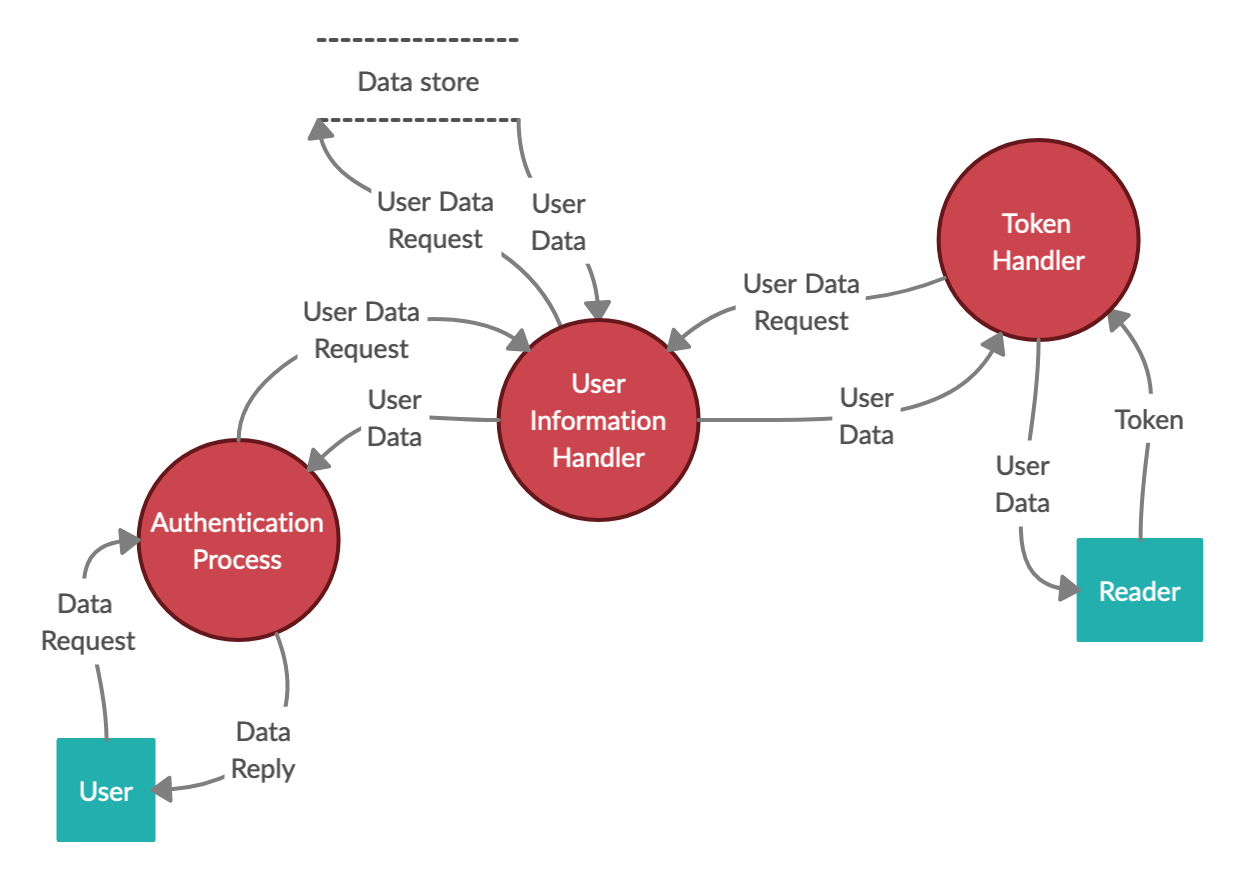
\includegraphics[width=0.7\linewidth]{img/backendDFD.png}
 	\caption{Backend Data Flow Diagram}
 \end{figure}
 
 We represented other elements of the system, such as the User and Reader, as external entities, in order to better exhibit our communication with them, and, the storage of the backend was displayed as a Data store.

\subsubsection{Finding Threats}

With our Data Flow Diagram done, we are now able to analyze it and find threats in a more streamlined way. In order to find the relevant threats, we will be using the STRIDE methodology:

\subsubsection{STRIDE}

\textbf{Spoofing}
\begin{itemize}
    \item When receiving a token from a supposed reader, we have no way of knowing if it was sent from a trusted source or not. In order to know if a token was sent from a reader and not an attacker, we should use a PKI\cite{pki}, so that every token has the signature of the reader who made the request, as well as the signature of the user whom information is being fetched.
    \item Considering the possibility of a backend user having his credentials stolen, an attacker is able to pose as one, and access our system. To prevent or hinder these kind of problems, it would be advised to implement a login system including \textbf{Two Factor Authentication}.
\end{itemize}

\textbf{Tampering}
\begin{itemize}
    \item As stated on the other entities, since we mostly rely on wireless communication, there exists the possibility of an attacker modifying data flowing over the network. To prevent this, a good idea would be to use TLS\cite{tls} and HTTPS for communications. With this, we could prevent an attacker from adding/modifying data that is being transmitted.
    \item If an attacker is able to enter into the operating system via spoofed credentials or lack of protection, the local Database can be compromised. These lack of specific protection could lead to an attacker being able to tamper with the information stored or make changes in the logs, compromising our system integrity. By implementing \textbf{Two Factor Authentication} and encrypting local data, we could prevent these unwanted activities, respectively.
\end{itemize}

\textbf{Repudiation}
\begin{itemize}
    \item Since we have no way of guaranteeing the authenticity of an entity's identity, we have no way of maintaining non-repudiation in our system. To get around that problem, and just like before, a PKI\cite{pki} would be useful to have signatures that uniquely identify an entity.
    \item Without keeping track of the transactions, from other entities, in a log, it's impossible for the system to guarantee that certain request came from an entity in particular. This could be solved adding a logging system that stores all the requests divided per entity.
    \item Changes to the system can be made without anyone knowing who it was. The system should have an encrypted logging system, in order to keep track of modifications and the responsible behind them. This would also help finding a compromised account.
\end{itemize}

\textbf{Information Disclosure}
\begin{itemize}
    \item The connection process with the other entities is done via TCP/IP. This technology allows an attacker to intercept the data being transmitted. To solve this, it's suggested the use of TLS\cite{tls} and HTTPS to provide integrity and privacy to the data being transmitted.
    \item The fact of not having any way of knowing the authenticity of an entity's identity, allows an attacker to pose as other entity in order to get information that otherwise wouldn't have access. This problem can be solved by implementing a PKI\cite{pki} to have signatures that uniquely identify an entity.
    \item Lack of authentication on the backend results in undesirable people having access to critical information. To solve this issue, it should be implemented a secure authentication method.
    \item In case of a process returning an error, an attacker can take advantage from this error message and extract information. 
    \item We also considered the possibility of a person being able to physically access the backend and steal information. This can't be fixed via software but is still possible. Although, strong data encryption could be implemented in order to make it more difficult. 
    \item Since the backend has a database, a set of bad permissions or configurations may lead to an attacker being able to explore the database without our consent. There should exist an effort to verify if the database has all configurations and permissions in order.
\end{itemize}

\textbf{Denial of Service}
\begin{itemize}
    \item An attacker with the objective of disrupting our service could try to flood the backend either with reader or user requests, occupying available resources. We could use the mentioned PKI\cite{pki} to discard requests with an invalid signature.
\end{itemize}

\textbf{Elevation of Privilege}
\begin{itemize}
    %\item Receive a request with code injetion in it for the purpose of execute code on the backend
    \item The lack of proper verification of the token received from supposed reader could give the possibility to an attacker to embed malicious code that can harm our system. Checking the tokens before doing anything with them is highly advised.
    %\item Lack of authentication results in unwanted people interacting with the managment part of the backend
    \item The lack of proper authentication in our system backend allows a potential attacker to access our backend and gain unwanted privileges within the system. This can be prevented by implementing a strong authentication system.
    \item The lack of encryption and access control to the data store of our backend allows an attacker to modify bits on disk to things other than what a backend user wants. This can be mitigated by encrypting local data.
    \item The lack of a firewall increases the odds of an attacker gaining unauthorized access to our system. By including a \textbf{firewall}\cite{firewall} to our system we could prevent this and also inspect more closely suspicious traffic.
    \item We also considered the possibility of a person being able to physically access the backend and run malicious code or gain privileged access. This can't be fixed via software but is still possible.
\end{itemize}

\subsubsection{CVE}

Since the system backend has specific specified, we used that to search for \textbf{CVE} that affect our system. Not only did we explore the current known vulnerabilities, but also vulnerabilities from the past. This approach will help to rectify ongoing problems and to be prepared for future threats.


\vspace{0.4cm}

\textbf{CentOS 7.8.2003}

The Operating System CentOS doesn't have many vulnerabilities at its core, and it couldn't be found any that was critical to our project. Although, some of the tools that can be used with this OS might have it, this problem gets out of our work scope, since the solution would vary with every tool. Before the use or installation of every program it should be made some search about past and current problems. Some of the  programs with problematic versions are CentOS Web Panel, Docker Engine and  Piranha Configuration Tool.


\vspace{0.4cm}

\textbf{PostgreSQL 12.1 \& PostgreSQL 12.4}

After a vast search of vulnerabilities which occurred over the past years with this \textbf{relational database management system} \textbf{(RDBMS)}, we managed to find some attack patterns. This threats normally took advantage of flawed commands and functions, code injections or badly defined user permission, these would allow the attacker to have access and modify data, or even shutdown the whole database. To prevent this developers should have special care with external functions and commands used, deal with external data with caution to avoid code injections and attention with the different users of the database and their permissions. The known CVEs to the versions that will be used are:

\textbf{CVE-2020-25695} - An attacker having permission to create non-temporary objects in at least one schema can execute arbitrary SQL functions under the identity of a superuser. The highest threat from this vulnerability is to data confidentiality and integrity as well as system availability.\cite{postgres1} \textbf{Updating to versions 12.5 or 13.1} fixes this issue. \textbf{This CVE has not CVSS score yet.}

\textbf{CVE-2020-25694} -  If a client application that creates additional database connections only reuses the basic connection parameters while dropping security-relevant parameters, an opportunity for a man-in-the-middle attack, or the ability to observe clear-text transmissions, could exist. The highest threat from this vulnerability is to data confidentiality and integrity as well as system availability.\cite{postgres2} \textbf{Updating to versions 12.5 or 13.1} fixes this issue. \textbf{This CVE has not CVSS score yet.}

\textbf{CVE-2020-14349} -  An authenticated attacker could use this flaw in an attack in order to execute arbitrary SQL command in the context of the user used for replication.\cite{postgres3} \textbf{Updating to version 12.4} fixes this issue. \textbf{This CVE has a CVSS score of 7.1, being classified as High.} This means that it is highly advised to fix it.


\vspace{0.4cm}

\textbf{Docker 19.03.6}

PostgreSQL has a Docker container running. Docker has some vulnerabilities specially if taking into account the runC container that is used by Docker. Most of the past vulnerabilities came from lack of content verification, such as code injection, spoofing, denial of service due to repeated join and quit actions, sharing of secrets on account of the debugging mode, being negligent on executing trojan horse programs and the use of commands as root to gain access to certain privileges and execute critical code. With this information we know that we need to be careful with how all external data is managed, and the use of some functionalities and commands.

\textbf{CVE-2020-13401} - An attacker in a container, with the CAP\_NET\_RAW capability, can craft IPv6 router advertisements, and consequently spoof external IPv6 hosts, obtain sensitive information, or cause a denial of service.\cite{docker1} \textbf{Updating to version 19.03.11} fixes this issue. \textbf{This CVE has a CVSS score of 6.0, being classified as Medium.} This means that it is advised to fix it, but not crucial.


\vspace{0.4cm}

\textbf{Ubuntu 20.04}

This version of Ubuntu is used for the management system of the backend. Despite being a stable version of this OS, there are still vulnerabilities to be found. In our search, we found out that most of the problems associated to this OS are related to utilities and tools that it ships with. Given the fact that we don't know if these tools will ever be used, we only considered CVE's directly related to the OS.

\textbf{CVE-2020-15708} - This CVE created a control socket with world read and write permissions. An attacker could use this to overwrite arbitrary files or execute arbitrary code.
\cite{ubuntu1} \textbf{This CVE has a CVSS score of 7.8, being classified as High.} This means that it is highly advised to fix it.


\vspace{0.4cm}

\textbf{Django v3.0}

The \textbf{Web Framework} Django has to deal with a lot of user input, because of this most of the vulnerabilities are related with lack of input validation, such as code, sql and malicious script tags injection, and key validation which can lead to data leakage. This problem can be mitigated, if from the beginning of the development of this project, all the input data is processed carefully. Some of the CVEs found to this version show this problem.

\textbf{CVE-2020-9402} - This allows SQL Injection if untrusted data is used as a tolerance parameter in GIS functions and aggregates on Oracle.\cite{django1} \textbf{Updating to version 3.0.4} fixes this issue. \textbf{This CVE has a CVSS score of 8.8, being classified as High.} This means that it is highly advised to fix it.

\textbf{CVE-2020-24584} - With this CVE, the intermediate-level directories of the filesystem cache had the system's standard umask rather than 0o077.\cite{django2} \textbf{Updating to version 3.0.10} fixes this issue. \textbf{This CVE has a CVSS score of 7.5, being classified as High.} This means that it is highly advised to fix it.

\textbf{CVE-2020-24583} - FILE\_UPLOAD\_DIRECTORY\_PERMISSIONS mode was not applied to intermediate-level directories created in the process of uploading files. It was also not applied to intermediate-level collected static directories when using the collectstatic management command. \cite{django3} \textbf{Updating to version 3.0.10} fixes this issue. \textbf{This CVE has a CVSS score of 7.5, being classified as High.} This means that it is highly advised to fix it.

\textbf{CVE-2020-13254} - In this CVE, In cases where a memcached backend does not perform key validation, passing malformed cache keys could result in a key collision, and potential data leakage. This can be solved \textbf{updating to version 3.0.7}.\cite{django4} \textbf{This CVE has a CVSS score of 5.9, being classified as Medium.}. If not possible updating to that version, it's important to have special care with key validation.

\textbf{CVE-2020-7471} - This vulnerability allows SQL Injection if untrusted data is used as a StringAgg delimiter. By passing a suitably crafted delimiter to a contrib.postgres.aggregates.StringAgg instance, it was possible to break escaping and inject malicious SQL.\cite{django5} This can be solved \textbf{updating to version 3.0.3}. \textbf{This CVE has a CVSS score of 9.8, being classified as Critical.}. This means that it is extremely advised to fix it.

\vspace{0.4cm}
\textbf{Flask 1.0}

Just like Django, Flask is a \textbf{Web Framework} and it has similar vulnerabilities issues. For the given version, it wasn't found any known vulnerability. Past vulnerabilities revolves around improper input validation and denial of service due to crafted encoded JSON data. Even though, this issues were solved in the current version, all data should be treated carefully.

\vspace{0.4cm}
\textbf{UWSGI \& Gunicorn}

UWSGI and Gunicorn are \textbf{Web Servers}. It's not explicit which version of them will be used, but these server didn't have many vulnerabilities in the past. These vulnerabilities are still important. They were based in flawed functions leading to overflows and return of wrong HTTP headers and inadequate calling and manipulation of files. To avoid this problems to happen in our project, we should have caution with the function used and code quality. 



\subsubsection{Risk Analysis}

With the help of the STRIDE methodology we were able to search for vulnerabilities that the backend may encounter when in operation. Unfortunately, resources are limited and there are vulnerabilities that are more important and should be addressed first. With that in mind, we tried to evaluate what should be implemented/focused on first. For that process of evaluation we tried to make a \textbf{Risk Analysis}, which involves analyzing the probability of something happening with the impact that is could have. We added also the weight of one solution fixing multiple problems and we also used the \textbf{CVE} of the listed version of software used to build the backend to have an idea of what kind problems could be more common.
Given this, and after making the proper analysis, we decided that from the previous solutions we proposed, the ones that should be focused on first are: the addition of a \textbf{Public Key Infrastructure} to the system, the use of \textbf{Transport Layer Security and HTTPS} in communications, the implementation of a \textbf{Firewall} and the implementation of an \textbf{input validation module}. Tanking into account the CVE's that we analyzed, we decided that input validation is critical and a strong firewall could mitigate some of them. By adding these functionalities to the system, a big part of the listed vulnerabilities could be mitigated.

\subsubsection{Official Emitting Entity}

%In our analysis we considered that the entity that provides user information and emits official documents is out of our scope, only considering that our backend has the information necessary in order to operate properly.

In our analysis we considered that the communication with the entity that provides user information and emits official documents is out of our scope, given that this communication would be entity dependent and would probably diversify a lot, so we considered that our backend has the information necessary in order to operate properly.

\pagebreak